% !TEX root=../dummy/dummy-06.tex

\section{第 \ref{sec.6.title} 章补充内容}

\subsection{对 HH132 数据集自旋极化体系准确性的讨论}
\label{sec.6.supp-HH132-remove}

在我们的测评与验证过程中,我们发现对于 HH132 数据集\cite{Hait-Head-Gordon.PCCP.2018}的 57 个自旋极化体系,其许多体系的计算本身存在挑战;我们的计算结果和 HH132 数据集的参考值与测评值也存在诸多差异。在正文中,我们仅对其中部分自旋极化体系作测评与统计;在这里,我们将详细地讨论复现 HH132 数据集过程中遇到的困难,并指出测评过程中剔除部分自旋极化体系的具体原因。

\subsubsection{对称性破缺}

\begin{table}[!t]
\centering
\caption[HH132 中存在对称性破缺问题的体系]{HH132 数据集中存在对称性破缺问题的分子及极化率结果${}^a$。}
\label{tab.6.supp.symm-broken}
\widetabular{
    \begin{tabular}{lld{4.4}d{2.3}d{2.3}d{2.3}d{2.3}d{2.3}}
    \toprule
    & & \multicolumn{3}{c}{解析极化率 / $\text{\AA}{}^{3}$\tnote{b}} & \multicolumn{3}{c}{HH132 原始数据 / $\text{\AA}{}^{3}$\tnote{c}} \\
    \cmidrule(lr){3-5} \cmidrule(lr){6-8}
    点群 & 体系 & \multicolumn{1}{c}{$\alpha_{xx}$} & \multicolumn{1}{c}{$\alpha_{yy}$} & \multicolumn{1}{c}{$\alpha_{zz}$} & \multicolumn{1}{c}{$\alpha_{xx}$} & \multicolumn{1}{c}{$\alpha_{yy}$} & \multicolumn{1}{c}{$\alpha_{zz}$} \\
    \midrule
    $SO(3)$                          & \ce{Be  } & 7.019      & 7.019    & 7.667   & 7.074      & 7.074     & 7.074     \\
    \midrule
    $D_{\infty h}$                   & \ce{Li2 } & 26.837     & 22.980   & 39.702  & 24.529     & 24.529    & 24.529    \\
    \midrule
    $C_{\infty v}$ & \ce{BN  } & 3.427      & 2.521    & 2.156   & 3.446      & 3.446     & 2.161     \\
    & \ce{NO  } & 1.444      & 1.240    & 0.434   & 1.445      & 1.445     & 0.557     \\
    & \ce{OCl } & 2.475      & 2.390    & 4.289   & 2.391      & 2.391     & 4.296     \\
    & \ce{OF  } & 1.057      & 1.081    & 1.814   & 1.057      & 1.057     & 1.816     \\
    & \ce{OH  } & 1.071      & 0.879    & 1.244   & 1.072      & 1.072     & 1.245     \\
    & \ce{SCl } & 4.065      & 4.387    & 7.137   & 4.393      & 4.393     & 7.147     \\
    & \ce{SF  } & 3.170      & 2.786    & 3.592   & 3.178      & 3.178     & 3.594     \\
    & \ce{SH  } & 2.875      & 3.449    & 3.446   & 3.458      & 3.458     & 3.450     \\
    & \ce{PS  } & 5.687      & 5.152    & 12.050  & 5.159      & 5.159     & 11.985    \\
    & \ce{NCO } & 2.264      & 2.232    & 4.005   & 2.233      & 2.233     & 4.028     \\
    \midrule
    $C_{3v}$                         & \ce{CH3O} & -318.402\tnote{d} & 2.644    & 3.326   & 4.080      & 2.762     & 3.330     \\
    \bottomrule
    \end{tabular}
}{
    \item[a] 表中所列的分子均为极化率张量 $\bm{\alpha}$ 不满足分子点群对称性的情形。列表中所展示的点群是分子构型对应的点群。计算模型是 MP2/aCVTZ。
    \item[b] 解析极化率由 \textsc{Gaussian 16} (rev B01)\cite{Gaussian16} 计算。该计算开启默认的对称性 (\ce{CH3O} 分子构型接近 $C_{3v}$,但程序中使用 $C_s$ 计算)。
    \item[c] 数据来自于 HH132 数据集原文\cite{Hait-Head-Gordon.PCCP.2018}。
    \item[d] \ce{CH3O} 自由基的解析 $\alpha_{xx}$ 分量数值确实存在异常;这在 \textsc{dh} 程序给出的结果中尽管具体数值不同,但也存在相当严重的误差。
}
\end{table}

在 HH132 的 57 个自旋极化分子中,13 个分子的电子态存在对称性破缺效应;因此解析极化率的计算与数值极化率有所不同。相关的数据列于表 \ref{tab.6.supp.symm-broken}。这些分子中,
\begin{itemize}[nosep]
    \item 以平均场的分子轨道讨论,\ce{BN}, \ce{NO}, \ce{OCl}, \ce{OF}, \ce{OH}, \ce{SCl}, \ce{SF}, \ce{SH}, \ce{PS}, \ce{NCO} 这 10 个 $C_{\infty v}$ 对称性自由基由于存在单电子占据的 $\Pi$ 不可约表示下的轨道,因此电子云在垂直于主轴的面上并不是均匀分布的 (即当主轴为 $z$ 轴时,电子云的分布在 $x$ 方向与 $y$ 方向并不相同)。依数值差分方法给出极化率,若电子占据轨道没有特定不可约表示的限制,那么在施加垂直于 $z$ 轴的外偶极电场时,电子云总是会旋转到能量更低的状态,而不是反映无外电场时的分布,因此会给出 $\alpha_{xx} = \alpha_{yy}$ 的结论;这也与 HH132 数据集的结果表现一致。但解析梯度给出的极化率可以反映无外电场时电子云的分布,即 $\alpha_{xx}$ 未必等于 $\alpha_{yy}$。我们认为,解析梯度的极化率是理论上严格的极化率计算方式;因此,我们决定在采用 HH132 数据集参考值时,排除这 10 个存在单电子占据的  $\Pi$ 不可约表示的 $C_{\infty v}$ 对称性自由基体系。
    \item 与上述原因类似地,我们排除 $C_{3v}$ 对称性下存在单电子占据 $E$ 不可约表示轨道的自由基 \ce{CH3O}。除此之外,该体系的解析极化率本身计算也容易产生数值问题。
    \item \ce{Be} 原子与 \ce{Li2} 分子则是在自洽场计算中,存在对称性更低、但能量上更稳定的态 (分别是 $C_{\infty v}$ 与 $C_s$);从而上述原因也会应用到这两个体系,导致不限制电子占据轨道不可约表示的数值极化率计算、与解析极化率在结果上存在差异。
\end{itemize}

\subsubsection{MP2 极化率复现问题}

\begin{table}[!t]
\centering
\caption[HH132 解析与数值极化率误差大的体系]{HH132 数据集解析与数值极化率相对误差超过 2\% 的体系、及其数值与误差${}^a$。}
\label{tab.6.supp.mp2-hait-g16}
\widetabular{
    \begin{tabular}{ld{3.3}d{3.3}d{3.3}d{4.4}d{4.4}d{4.4}}
    \toprule
    & \multicolumn{3}{c}{解析极化率 / $\text{\AA}{}^{3}$\tnote{b}} & \multicolumn{3}{c}{相对误差 / \%\tnote{c}} \\
    \cmidrule(lr){2-4} \cmidrule(lr){5-7}
    体系 & \multicolumn{1}{c}{$\alpha_{xx}$} & \multicolumn{1}{c}{$\alpha_{yy}$} & \multicolumn{1}{c}{$\alpha_{zz}$} & \multicolumn{1}{c}{$\alpha_{xx}$} & \multicolumn{1}{c}{$\alpha_{yy}$} & \multicolumn{1}{c}{$\alpha_{zz}$} \\
    \midrule
    \ce{CH2NH} & 3.299    & 2.713    & 6.678    & 0.129       & 0.191      & -115.065    \\
    \ce{HOF  } & 1.443    & 1.254    & 4.023    & 0.028       & 0.061      & -40.274     \\
    \ce{NOCl } & 5.814    & 6.487    & 3.452    & -67.820     & -8.420     & 0.075       \\
    \ce{Na2  } & 30.066   & 30.066   & 26.148   & 0.069       & 0.069      & 2.452       \\
    \ce{NaLi } & 26.443   & 26.443   & -11.852  & 0.100       & 0.100      & -18.332     \\
    \bottomrule
    \end{tabular}
}{
    \item[a] 该表格的分析中,去除了表 \ref{tab.6.supp.symm-broken} 所涉及的 13 个分子。计算模型是 MP2/aCVTZ。
    \item[b] 解析极化率由 \textsc{Gaussian 16} (rev B01)\cite{Gaussian16} 计算。
    \item[c] 相对误差是指 HH132 数值极化率相对于 \textsc{Gaussian 16} 计算得到的解析极化率的比值误差。
}
\end{table}

\begin{table}[!ht]
\centering
\caption[HH132 不同程序解析极化率误差大的体系]{HH132 数据集不同程序 (\textsc{dh} 与 \textsc{Gaussian 16}) 解析极化率相对误差超过 0.5\% 的体系、及其数值与误差${}^a$。}
\label{tab.6.supp.mp2-dh-g16}
\widetabular{
    \begin{tabular}{ld{3.3}d{3.3}d{3.3}d{3.3}d{3.3}d{3.3}}
    \toprule
    & \multicolumn{3}{c}{解析极化率 / $\text{\AA}{}^{3}$\tnote{b}} & \multicolumn{3}{c}{相对误差 / \%\tnote{c}} \\
    \cmidrule(lr){2-4} \cmidrule(lr){5-7}
    体系 & \multicolumn{1}{c}{$\alpha_{xx}$} & \multicolumn{1}{c}{$\alpha_{yy}$} & \multicolumn{1}{c}{$\alpha_{zz}$} & \multicolumn{1}{c}{$\alpha_{xx}$} & \multicolumn{1}{c}{$\alpha_{yy}$} & \multicolumn{1}{c}{$\alpha_{zz}$} \\
    \midrule
    \ce{CH2NH} & 3.299  & 2.713  & 6.678   & 0.160 & 0.073  & 22.152 \\
    \ce{NOCl } & 5.814  & 6.487  & 3.452   & 4.268 & 4.564  &  0.017 \\
    \ce{NaLi } & 26.443 & 26.443 & -11.852 & 0.225 & 0.225  & -9.846 \\
    \bottomrule
    \end{tabular}
}{
    \item[a] 该表格的分析中,去除了表 \ref{tab.6.supp.symm-broken} 所涉及的 13 个分子。计算模型是 MP2/aCVTZ。\textsc{dh} 程序计算结果使用 ETB 辅助基组。
    \item[b] 解析极化率由 \textsc{Gaussian 16} (rev B01)\cite{Gaussian16} 计算。
    \item[c] 相对误差是 \textsc{dh} 计算得到的解析极化率、相对于 \textsc{Gaussian 16} 计算得到的解析极化率的比值误差。
}
\end{table}

通过解析梯度计算复现 HH132 数据集的 MP2/aCVTZ 数值极化率数据时,我们认为部分体系误差较大。其中,由 \textsc{Gaussian 16} 解析计算的极化率与 HH132 原始数据集中存在大于 2\% 差异的体系有 5 个,如表 \ref{tab.6.supp.mp2-hait-g16} 所示。这些分子中,\ce{CH2NH}, \ce{NOCl}, \ce{NaLi} 使用不同的程序下给出的解析极化率也有一定程度上的不同,如表 \ref{tab.6.supp.mp2-dh-g16} 所示;这表明这些分子的电子云在 MP2/aCVTZ 模型下并不稳定,其极化率容易受外场或数值精度的影响而产生大幅改变。由于 HH132 数据集中的 MP2 极化率结果是 CCSD(T) 参考值结果的中间输出,因此我们认为,若 MP2 的计算偏差较大、那么作为参考值的 CCSD(T) 也很可能存在无法忽视的偏差;从而这些分子体系不适合使用 HH132 的参考值对诸泛函作测评。

\subsubsection{其他双杂化泛函复现或数值问题}

\begin{table}[!htp]
\centering
\caption[HH132 双杂化泛函 aCVTZ 数值与解析极化率误差大体系]{HH132 数据集部分双杂化泛函 aCVTZ 数值与解析极化率相对误差超过 2\% 的体系、及其数值与误差${}^a$。}
\label{tab.6.supp.double-hybrid-hh132-g16}
\widetabular{
    \begin{tabular}{llld{1.3}d{1.3}d{1.3}d{3.3}d{3.3}d{3.3}}
    \toprule
    & & & \multicolumn{3}{c}{解析极化率 / $\text{\AA}{}^{3}$\tnote{b}} & \multicolumn{3}{c}{相对误差 / \%\tnote{c}} \\
    \cmidrule(lr){4-6} \cmidrule(lr){7-9}
    泛函 & 体系 & 自旋极化 & \multicolumn{1}{c}{$\alpha_{xx}$} & \multicolumn{1}{c}{$\alpha_{yy}$} & \multicolumn{1}{c}{$\alpha_{zz}$} & \multicolumn{1}{c}{$\alpha_{xx}$} & \multicolumn{1}{c}{$\alpha_{yy}$} & \multicolumn{1}{c}{$\alpha_{zz}$} \\
    \midrule
    B2PLYP & \ce{C2H  } & SP  & 3.543 & 3.543 & 4.020  & 8.564   & 8.564   & -0.127  \\
    53\% $E_\textmt{x}^\mathrm{exact}$ & \ce{CN   } & SP  & 3.192 & 3.192 & 4.518  & -18.839 & -18.839 & -2.985  \\
    & \ce{HNS  } & SP  & 5.796 & 3.959 & 3.031  & -1.502  & 3.246   & 10.542  \\
    & \ce{NaCl } & NSP & 4.334 & 4.334 & 5.471  & 0.698   & 0.698   & 2.058   \\
    & \ce{O3   } & SP  & 1.713 & 4.580 & 2.124  & 0.000   & -4.345  & -1.471  \\
    \midrule
    B2GPPLYP      & \ce{C2H  } & SP  & 3.395 & 3.395 & 4.009  & 7.009   & 7.009   & -0.751  \\
    65\% $E_\textmt{x}^\mathrm{exact}$ & \ce{CN   } & SP  & 3.304 & 3.304 & 4.243  & -18.696 & -18.696 & -1.834  \\
    & \ce{HNO  } & SP  & 1.490 & 2.289 & 2.719  & 5.253   & 0.786   & 1.883   \\
    & \ce{HNS  } & SP  & 6.974 & 3.971 & 4.786  & -18.989 & 1.673   & -30.387 \\
    & \ce{NP   } & SP  & 3.357 & 3.357 & 6.635  & 6.480   & 6.480   & -18.120 \\
    & \ce{O2   } & SP  & 1.174 & 1.174 & 2.193  & 0.372   & 0.372   & -3.047  \\
    & \ce{O3   } & SP  & 1.696 & 4.518 & 2.095  & 0.226   & -4.981  & -1.451  \\
    \midrule
    DSD-PBEPBE-D3 & \ce{BO   } & SP  & 2.308 & 2.308 & 2.790  & 0.141   & 0.141   & 3.479   \\
    69\% $E_\textmt{x}^\mathrm{exact}$ & \ce{BS   } & SP  & 4.437 & 4.437 & 6.279  & -0.390  & -0.390  & 2.786   \\
    & \ce{C2H  } & SP  & 3.275 & 3.275 & 4.028  & 5.621   & 5.621   & -2.152  \\
    & \ce{C2H3 } & SP  & 3.458 & 5.224 & 3.253  & -0.041  & -2.868  & -1.886  \\
    & \ce{CH2PH} & SP  & 9.288 & 5.237 & 5.774  & -18.140 & -4.902  & -1.666  \\
    & \ce{CN   } & SP  & 3.168 & 3.168 & 3.985  & -14.950 & -14.950 & 0.268   \\
    & \ce{F2   } & SP  & 0.886 & 0.886 & 2.649  & 2.027   & 2.027   & -32.081 \\
    & \ce{HNO  } & SP  & 1.373 & 2.288 & 2.662  & 13.702  & 0.703   & 3.008   \\
    & \ce{HNS  } & SP  & 6.957 & 3.972 & 3.554  & -19.780 & 1.397   & -6.832  \\
    & \ce{NP   } & SP  & 3.320 & 3.320 & 6.949  & 7.205   & 7.205   & -22.109 \\
    & \ce{O2   } & SP  & 1.179 & 1.179 & 2.236  & 0.584   & 0.584   & -3.005  \\
    & \ce{O3   } & SP  & 1.697 & 4.495 & 2.096  & -0.148  & -7.296  & -1.446  \\
    & \ce{P2   } & SP  & 6.176 & 6.176 & 11.026 & -3.827  & -3.827  & -7.977  \\
    \bottomrule
    \end{tabular}
}{
    \item[a] 该表格的分析中,去除了表 \ref{tab.6.supp.symm-broken} 所涉及的 13 个分子和表 \ref{tab.6.supp.mp2-hait-g16} 所涉及的 5 个分子;即总共涉及 HH132 数据集中的 114 个分子,其中自旋极化分子数为 44 个。
    \item[b] 解析极化率由 \textsc{Gaussian 16} (rev B01)\cite{Gaussian16} 计算。基组为 aCVTZ、DFT 积分格点选用程序默认的格点。
    \item[c] 相对误差是指 HH132 数值极化率相对于 \textsc{Gaussian 16} 计算得到的解析极化率的比值误差。
}
\end{table}

Hait 与 Head-Gordon 在 HH132 数据集上测评了双杂化泛函\cite{Hait-Head-Gordon.PCCP.2018};他们汇报了这些双杂化泛函的 aCVTZ 基组计算结果。其中,B2PLYP、B2GPPLYP、DSD-PBEPBE-D3 三种泛函也可以通过 \textsc{Gaussian 16} 作对比验证。对比的结果如表 \ref{tab.6.supp.double-hybrid-hh132-g16} 所示。从表中可以看出,B2PLYP 下的 \ce{NaCl} 作为自旋非极化分子,其误差尽管超过 2\% 但也未超过 3\%。但其余表格中涉及到的分子,有许多误差超过 5\% 或更大;这种程度的误差将对测评结果产生明显影响。我们也注意到这些分子几乎全部是自旋极化分子,其较大的误差、较有可能来自于电子态的收敛结果不同。事实上,我们在 \textsc{Gaussian 16} 解析极化率计算中采用的稳定性分析 (stability analysis) 是基于 aCVTZ 基组、而 HH132 测评工作大多数情况下基于 aug-pc-2 基组\cite{Hait-Head-Gordon.PCCP.2018};尽管这两个基组的大小较为接近,但仍然是不同的基组,确实在一些分子下可能导致波函数的稳定性有所差异。同时我们观察到,泛函中交换系数较高时,极化率出现较大偏差的分子也较多、波函数也更有可能不稳定;这种现象也出现在偶极矩计算问题中\cite{Gu-Xu.JCTC.2021a}。

我们也使用 \textsc{dh} 程序作 HH132 数据集 B2PLYP、B2GPPLYP、DSD-PBEPBE-D3 泛函在 aCVTZ 下极化率的验证计算。大部分分子的计算结果与 \textsc{Gaussian 16} 数值上非常接近;所有误差大于 0.2\% 的体系列表于 \ref{tab.6.supp.double-hybrid-dh-g16};即使极少数分子确实存在误差,但误差最大也不超过 1\%。在排除对称性破缺的 13 个体系、以及 MP2 复现问题的 5 个体系后,\textsc{dh} 程序与 \textsc{Gaussian 16} 几乎给出完全一致的解析极化率,从而也基本验证了 \textsc{dh} 程序的正确性、也同时验证了 \textsc{Gaussian 16} 所计算得到的数据可以由其他程序复现。

\begin{table}[!t]
\centering
\caption[HH132 双杂化泛函 aCVTZ 数据不同程序解析极化率误差大的体系]{HH132 数据集部分双杂化泛函 aCVTZ 数据不同程序 (\textsc{dh} 与 \textsc{Gaussian 16}) 解析极化率相对误差超过 0.2\% 的体系、及其数值与误差${}^a$。}
\label{tab.6.supp.double-hybrid-dh-g16}
\widetabular{
    \begin{tabular}{llld{2.3}d{2.3}d{2.3}d{2.3}d{2.3}d{2.3}}
    \toprule
    & & & \multicolumn{3}{c}{解析极化率 / $\text{\AA}{}^{3}$\tnote{b}} & \multicolumn{3}{c}{相对误差 / \%\tnote{c}} \\
    \cmidrule(lr){4-6} \cmidrule(lr){7-9}
    泛函 & 体系 & 自旋极化 & \multicolumn{1}{c}{$\alpha_{xx}$} & \multicolumn{1}{c}{$\alpha_{yy}$} & \multicolumn{1}{c}{$\alpha_{zz}$} & \multicolumn{1}{c}{$\alpha_{xx}$} & \multicolumn{1}{c}{$\alpha_{yy}$} & \multicolumn{1}{c}{$\alpha_{zz}$} \\
    \midrule
    B2PLYP        & \ce{LiCl} & NSP & 3.894 & 3.894 & 4.194 & 0.051  & 0.051  & 0.245  \\ \midrule
    B2GPPLYP      & \ce{NP  } & SP  & 3.357 & 3.357 & 6.635 & 0.000  & 0.000  & 0.812  \\
                  & \ce{NaH } & NSP & 5.326 & 5.326 & 7.562 & -0.515 & -0.515 & -0.041 \\ \midrule
    DSD-PBEPBE-D3 & \ce{LiH } & NSP & 4.282 & 4.282 & 3.767 & -0.203 & -0.203 & -0.055 \\
    \bottomrule
    \end{tabular}
}{
    \raggedright
    \item[a] 该表格的分析中,去除了表 \ref{tab.6.supp.symm-broken} 所涉及的 13 个分子和表 \ref{tab.6.supp.mp2-hait-g16} 所涉及的 5 个分子;即总共涉及 HH132 数据集中的 114 个分子,其中自旋极化分子数为 44 个。\textsc{dh} 程序计算结果使用 ETB 辅助基组。
    \item[b] 解析极化率由 \textsc{Gaussian 16} (rev B01)\cite{Gaussian16} 计算。基组为 aCVTZ、DFT 积分格点选用程序默认的格点。
    \item[c] 相对误差是指 HH132 数值极化率相对于 \textsc{Gaussian 16} 计算得到的解析极化率的比值误差。
}
\end{table}

总地来说,自旋极化体系的极化率计算结果容易因对称性破缺、收敛问题、波函数稳定性问题、外加电场合理性问题等等,而导致不同程序、不同计算策略会给出不同的结果。表 \ref{tab.6.supp.double-hybrid-hh132-g16} 涉及到的自旋极化体系的数量有 13 个;加上表 \ref{tab.6.supp.symm-broken} 涉及到的 13 个对称性破缺体系、与表 \ref{tab.6.supp.mp2-hait-g16} 涉及到的 5 个 MP2 极化率误差超过 2\% 的体系,总共有 31 个自旋极化体系的计算存在困难。这占到 HH132 数据集中 57 个自旋极化体系的 54\%。

一方面,为尽可能保证测评的公平,我们将在 HH132 数据集的计算中,排除上述计算上有困难的 31 个自旋极化体系;即对 HH132 数据集总共测评 101 个分子,记为 HH101 数据集;其中自旋非极化体系为 75 个保持不变、自旋极化体系为 26 个。具体计算的体系如 \ref{tab.6.supp.HH101-species} 所示。另一方面,由于排除的自旋极化体系过多,很大程度上改变了原先数据集自旋极化与非极化体系的平衡;因此与 HH132 测评工作\cite{Hait-Head-Gordon.PCCP.2018}不同,本工作的测评结果将对自旋极化与非极化体系分别作测评,而不测评两类体系的总误差。

\begin{table}[!htp]
\centering
\caption[本工作所测评的 HH101 数据集体系]{本工作所测评的 HH101 数据集体系;其中自旋极化体系 75 个、自旋极化体系 26 个。}
\label{tab.6.supp.HH101-species}
\widetabular{
    \begin{tabular}{llllllll}
    \toprule
    \multicolumn{6}{c}{NSP} & \multicolumn{2}{c}{SP} \\
    \cmidrule(lr){1-6} \cmidrule(lr){7-8}
    \ce{AlF   } & \ce{CH3F  } & \ce{FNO   } & \ce{HF   } & \ce{NH2Cl} & \ce{PH3O  } & \ce{^2BH2   } & \ce{^2Li  } \\
    \ce{Ar    } & \ce{CH3NH2} & \ce{^2H   } & \ce{HNC  } & \ce{NH2F } & \ce{S2H2  } & \ce{^2BeH   } & \ce{^4N   } \\
    \ce{BF    } & \ce{CH3OH } & \ce{H2    } & \ce{HOCl } & \ce{NH2OH} & \ce{SCl2  } & \ce{^3CH2   } & \ce{^1N2H2} \\
    \ce{BH2Cl } & \ce{CH3SH } & \ce{H2O   } & \ce{HOOH } & \ce{NH3  } & \ce{SF2   } & \ce{^2CH2F  } & \ce{^3NH  } \\
    \ce{BH2F  } & \ce{CH4   } & \ce{HBO   } & \ce{He   } & \ce{NH3O } & \ce{SH2   } & \ce{^2CH3   } & \ce{^2NH2 } \\
    \ce{BH3   } & \ce{CO    } & \ce{HBS   } & \ce{LiBH4} & \ce{NaCN } & \ce{SO2   } & \ce{^2FCO   } & \ce{^2Na  } \\
    \ce{BHF2  } & \ce{CO2   } & \ce{HCCCl } & \ce{LiCN } & \ce{NaCl } & \ce{SiH3Cl} & \ce{^2FH-OH } & \ce{^1OF2 } \\
    \ce{BeH2  } & \ce{CS    } & \ce{HCCF  } & \ce{LiCl } & \ce{NaH  } & \ce{SiH3F } & \ce{^2H2CN  } & \ce{^4P   } \\
    \ce{C2H2  } & \ce{CSO   } & \ce{HCHO  } & \ce{LiH  } & \ce{Ne   } & \ce{SiH4  } & \ce{^2H2O-Li} & \ce{^3PH  } \\
    \ce{C2H4  } & \ce{Cl2   } & \ce{HCN   } & \ce{Mg   } & \ce{OCl2 } & \ce{SiO   } & \ce{^1HCHS  } & \ce{^2PH2 } \\
    \ce{CH2BH } & \ce{ClCN  } & \ce{HCONH2} & \ce{Mg2  } & \ce{P2H4 } & \ce{      } & \ce{^2HCO   } & \ce{^3S2  } \\
    \ce{CH3BH2} & \ce{ClF   } & \ce{HCOOH } & \ce{N2   } & \ce{PH2OH} & \ce{      } & \ce{^1HCP   } & \ce{^3SO  } \\
    \ce{CH3Cl } & \ce{FCN   } & \ce{HCl   } & \ce{N2H4 } & \ce{PH3  } & \ce{      } & \ce{^2HO2   } & \ce{^2SiH3} \\
    \bottomrule
    \end{tabular}
}{}
\end{table}

\subsection{HH101 数据集下 B2PLYP 极化率分量的相对误差分析}

表 \ref{tab.6.b2p-conv-hh101-rmsre} 展示了 HH101 数据集下 B2PLYP 在极化率分量 $\alpha_{xx}, \alpha_{yy}, \alpha_{zz}$ 下的基组收敛性表现。这里的误差计算方式与 Hait 等\cite{Hait-Head-Gordon.PCCP.2018}在 HH132 测评过程中所使用的标准 RMSRE 相匹配。该表格与表 \ref{tab.6.b2p-conv-hh101-iso} 相同,均是考察 HH101 数据集下 B2PLYP 极化率的基组收敛性。由于 HH101 数据集本身只包含三个极化率分量 $\alpha_{xx}$, $\alpha_{yy}$, $\alpha_{zz}$,而该数据集部分分子的极化率张量非对角元 $\alpha_{xy}$, $\alpha_{yz}$, $\alpha_{zx}$ 非零,从而尚无各向异性极化率 $\gamma$。因此,表 \ref{tab.6.b2p-conv-hh101-rmsre} 对三个极化率张量对角元分量的考量,能体现极化率非同性效应的基组收敛性。对比表 \ref{tab.6.b2p-conv-hh101-iso},我们认为在相同的基组下,对极化率张量的对角元分量 $\alpha_{xx}$, $\alpha_{yy}$, $\alpha_{zz}$ 的基组相对误差比同性极化率 $\alpha$ 的误差更大,但变化幅度不大、且误差趋势一致。因此,我们认为正文对同性极化率 $\alpha$ 的基组误差分析结论,也可以应用于对角元分量 $\alpha_{xx}$, $\alpha_{yy}$, $\alpha_{zz}$ 的分析中。

\begin{table}[!ht]
\centering
\caption[B2PLYP 在数据集 HH101 下极化率分量基组 RelRMSD]{B2PLYP 在数据集 HH101 下极化率分量 $\alpha_{xx}, \alpha_{yy}, \alpha_{zz}$ 的基组相对方均根误差 (RelRMSD / \%)${}^a$。}
\label{tab.6.b2p-conv-hh101-rmsre}
\widetabular{
    \begin{tabular}{cld{1.3}d{1.3}d{1.3}d{1.3}d{1.3}d{1.3}}
    \toprule
    & & \multicolumn{3}{c}{HH101 (NSP)\tnote{b}} & \multicolumn{3}{c}{HH101 (SP)} \\
    \cmidrule(lr){3-5} \cmidrule(lr){6-8}
    基组 & 基组基数 & \multicolumn{1}{c}{$\tilde \alpha_\textsf{SCF}$} & \multicolumn{1}{c}{$\symup{\Delta} \tilde \alpha_\textsf{PT2}$} & \multicolumn{1}{c}{$\tilde \alpha_\textsf{DH}$} & \multicolumn{1}{c}{$\tilde \alpha_\textsf{SCF}$} & \multicolumn{1}{c}{$\symup{\Delta} \tilde \alpha_\textsf{PT2}$} & \multicolumn{1}{c}{$\tilde \alpha_\textsf{DH}$} \\
    \midrule
    2-$\zeta$ & aCVDZ    & 4.990 & 0.619 & 5.390 & 4.276 & 0.815 & 4.673 \\
              & apc1     & 2.069 & 0.900 & 2.278 & 1.804 & 0.962 & 1.934 \\ \midrule
    3-$\zeta$ & aCVTZ    & 1.455 & 0.324 & 1.690 & 1.019 & 0.364 & 1.211 \\
              & apc2     & 0.607 & 0.349 & 0.561 & 0.656 & 0.628 & 0.712 \\
              & aCV[DT]Z &       & 0.240 & 1.584 &       & 0.240 & 1.104 \\
              & apc[12]  &       & 0.560 & 0.674 &       & 0.516 & 0.632 \\ \midrule
    4-$\zeta$ & aCVQZ    & 0.323 & 0.166 & 0.468 & 0.181 & 0.218 & 0.331 \\
              & apc3     & 0.214 & 0.181 & 0.302 & 0.182 & 0.146 & 0.202 \\
              & aCV[TQ]Z &       & 0.077 & 0.370 &       & 0.163 & 0.250 \\
              & apc[23]  &       & 0.343 & 0.410 &       & 0.231 & 0.354 \\ \midrule
    5-$\zeta$ & aCV5Z    & \multicolumn{1}{c}{0} & 0.085 & 0.085 & \multicolumn{1}{c}{0} & 0.112 & 0.112 \\
              & apc4     & 0.238 & 0.078 & 0.279 & 0.160 & 0.114 & 0.210 \\
              & aCV[Q5]Z &       & \multicolumn{1}{c}{0} & \multicolumn{1}{c}{0} &       & \multicolumn{1}{c}{0} & \multicolumn{1}{c}{0} \\
              & apc[34]  &       & 0.214 & 0.335 &       & 0.097 & 0.199 \\
    \bottomrule
    \end{tabular}
}{
    \item[a] 该表格的图例参考表 \ref{tab.6.b2p-conv-hr46-t144-iso}。极化率分量的相对方均根误差公式也可以参考式 (\ref{eq.6.rmsre})。
    \item[b] 由于氢原子在 \textsc{dh} 程序中无法给出解析极化率,因此分析自旋非极化分子总体误差时排除氢原子,即总共分析 74 个自旋非极化体系。
}
\end{table}

\subsection{极化率基组不完备性补充推测与推论}
\label{sec.6.supp-bsie}

在正文中,所有基组误差与收敛性分析是基于 aCV[Q5]Z 外推模型作为参考而来;而 aCV[Q5]Z 作为非常精确且昂贵的外推模式,已经应用于 HH132 数据集的构建\cite{Hait-Head-Gordon.PCCP.2018},是目前流行且受到承认的高精度基组模型。

但也必须指出,对于 aCV[Q5]Z 本身 BSIE 的具体数值,目前的研究较少。一方面,尚不完全明朗的 aCV[Q5]Z 外推模型的 BSIE 意味着 HH132 数据集参考值\cite{Hait-Head-Gordon.PCCP.2018}、第 \alertref{sec.5.title} 章所述的 HR46 与 T144 数据集参考值除了 CCSD(T) 方法本身的误差外,仍然存在一定的 BSIE 且具体的数值尚无定量估计,即参考值的可信度仍然有提升空间。另一方面,基组极限下的计算量是巨大的;而使用巨大的 Gaussian 函数型基组还可能容易导致对角化算法或部分电子积分在双浮点精度下出现数值问题。在静态极化率的计算问题上,Brakestad 等人\cite{Brakestad-Frediani.JCTC.2020}通过多重小波 (MW) 基组方法,有效地对 PBE、VWN 方法逼近基组极限;但该工作测评的 Gaussian 函数型基组仅包含 apc4 而未考察其他基组、同时 MW 型基组难以简单推广到后自洽场方法或双杂化泛函近似。因此,CCSD(T)/aCV[Q5]Z 的 BSIE 数值、以及接近基组极限的自洽场方法或双杂化泛函静态极化率计算,目前还存在技术上的困难。

由于上述困难,严格的 BSIE 分析目前无法实现。但通过对现有数据的分析,我们可以作一些猜测与推论。这些猜测与推论将不会明显影响正文中对 apc3 基组误差的论断,也不会弱化使用 apc3 作双杂化泛函静态极化率测评的合理性。

\subsubsection{aCV$\bm{X}$Z 与 apc$\bm{n}$ 基组函数构成的比较。}

我们首先比较 3,4,5-$\zeta$ 基组基数下,aCV$X$Z ($X=\mathrm{T,Q,5}$) 与 apc$n$ ($n=2,3,4$) 基组函数的构成。图 \ref{fig.6.basis-exponent-plot} 展示了这两类基组的碳原子原始 GTO 函数指数分布、以及它们是否单独构成基组或缩并为 CGTO。可以看到,apc$n$ 基组系列在靠近原子核的区域 (原始 GTO 函数的指数较大的区域) 仅使用少量 $s, p$ 壳层的 CGTO 基组描述;而 aCV$X$Z 基组系列则在指数为 5--125 的区域内依基组基数的,引入 $s, p, d, f, g$ 壳层的原始 GTO 函数作为基组。在不靠近原子核的区域 (原始 GTO 函数指数小于 5 的区域),两类基组都使用原始 GTO 函数作为基函数,apc$n$ 的 GTO 函数指数分散程度比 aCV$X$Z 更宽。在相同的基组基数下,apc$n$ 的 GTO 函数指数的最低数值 (最弥散的基函数) 也比 aCV$X$Z 更低 (更加弥散);这点在更大的基组、更高的角动量壳层下尤为明显。

\begin{figure}[!t]
    \centering
    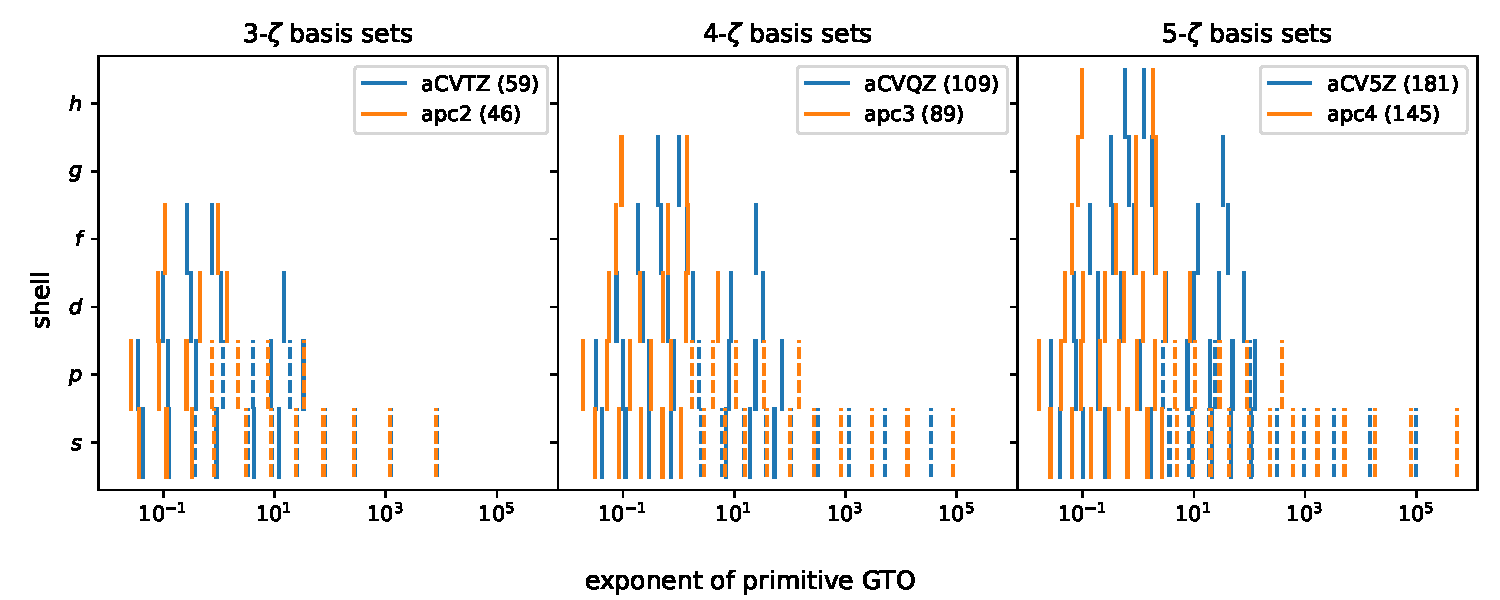
\includegraphics[width=0.9\textwidth]{assets/basis_exponent_plot.pdf}
    \caption[aCV$X$Z 与 apc$n$ 碳原子基函数构成]{aCV$X$Z ($X=\mathrm{T,Q,5}$) 与 apc$n$ ($n=2,3,4$) 碳原子基函数构成。线条对应的横坐标是 GTO 的指数。实线对应的是作为基函数的原始 GTO。虚线对应的是 CGTO 中被缩并的原始 GTO;单根虚线不构成基。缩并系数信息未展示于该图。图例括号中的数字代表该基组碳原子的基函数数量。}
    \label{fig.6.basis-exponent-plot}
\end{figure}

当对比 apc$n$ ($n=2,3,4$) 与 aCV5Z 时,如图 \ref{fig.6.basis-exponent-plot-compare} 所示,可以发现每个壳层下,apc$n$ 基组的弥散函数普遍比 aCV5Z 更加弥散 (除了 apc2 在 $d$ 壳层的弥散基组)。aCV5Z 相对于 apc$n$ 来说,则是增加了靠近原子核区域的原始 GTO 基函数、以及在价层区域有更为密集的原始 GTO 基函数。

\begin{figure}[!t]
    \centering
    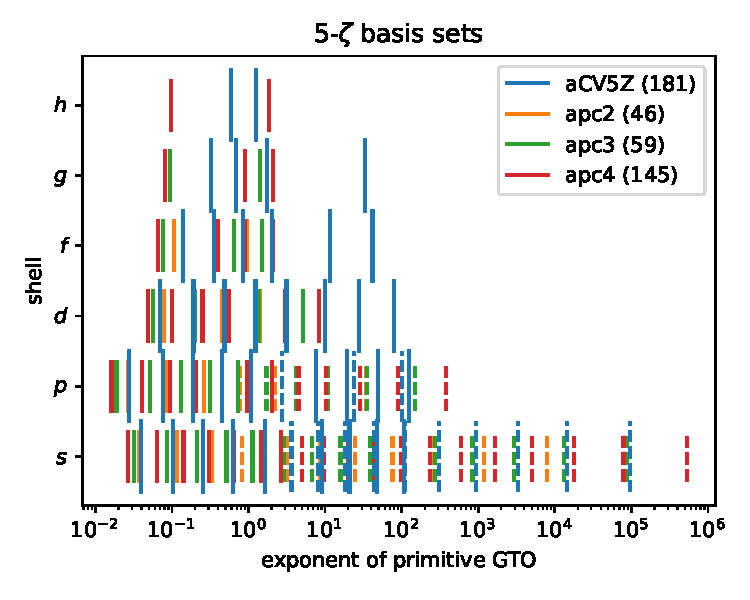
\includegraphics[width=0.4\textwidth]{assets/basis_exponent_plot_compare.pdf}
    \caption[aCV5Z 与 apc$n$ 碳原子基函数构成]{aCV5Z 与 apc$n$ ($n=2,3,4$) 碳原子基函数构成。图例参考图 \ref{fig.6.basis-exponent-plot}。}
    \label{fig.6.basis-exponent-plot-compare}
\end{figure}

\subsubsection{B2PLYP 同性极化率中自洽场泛函部分 $\alpha_\textsf{SCF}$ 的收敛趋势}

这一小节中,为简化分析,我们仅细致考察同性极化率 $\alpha$ 的基组收敛趋势。接续 \ref{sec.6.basis-converg} 节的做法,作为双杂化的典型泛函的典型,我们对 B2PLYP 的基组收敛趋势作详细分析。由于自洽场部分 $\alpha_\textsf{SCF}$ 与微扰部分 $\symup{\Delta} \alpha_\textsf{PT2}$ 的收敛趋势并不相同,因此两个贡献部分将分开讨论。

这里的分析将使用小提琴图 (violin plot)。该图像的纵坐标轴是双对数 (symmetric logarithmic) 缩放,线性区间为 $-0.01$\% 至 $0.01$\%;图像的数据密度建模方式是 Gaussian 核,采样的数据是纵坐标轴缩放后的结果 (而非误差本身),模型参数设为较小的 \texttt{bw\_method=0.1}。图像纵坐标的主格点是 $\pm 10^{n} \%$ $(n = -2, -1, 0, 1)$,副格点是 $\pm 5 \times 10^{n} \%$ $(n = -2, -1, 0)$。该类型图可以展示数据分布的细节,但当前的绘制方式不会凸显较为异常的数值;相对地,正文中的相对方均根误差 RelRMSD 对误差较大的数据比较敏感,两种分析可以互补。同时,小提琴图展示的是误差分布本身,而非每个数据点的误差随着基组增大而变化的趋势;因此仍然无法分析具体分子或某一类分子的基组收敛趋势。

\begin{figure}[!t]
    \centering
    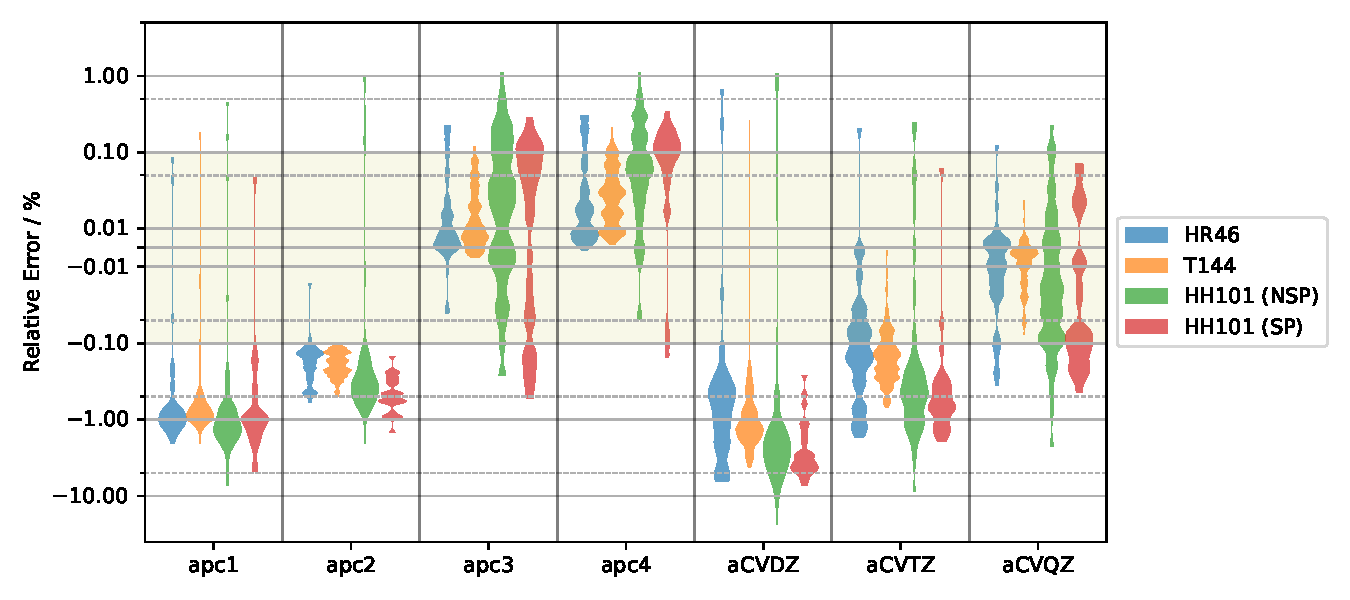
\includegraphics[width=0.9\textwidth]{assets/converg-b2p-scf-aCV5Z.pdf}
    \caption[B2PLYP $\alpha_\textsf{SCF}$ 不同基组相对于 aCV5Z 的相对误差]{B2PLYP 同性极化率的自洽场贡献部分 $\alpha_\textsf{SCF}$ 不同基组相对于 aCV5Z 的相对误差。对于 HH101 非自旋极化数据集 (NSP),氢原子未纳入该图的分析 (下同)。}
    \label{fig.6.converg-b2p-scf-aCV5Z}
\end{figure}

图 \ref{fig.6.converg-b2p-scf-aCV5Z} 展示的是当选取 aCV5Z 基组作为参考值时,B2PLYP 自洽场部分同性极化率 $\alpha_\textsf{SCF}$ 在不同基组下的相对误差。总体来说,基组越大,误差分布大体上越接近零点附近;这意味着 aCV5Z 基组确实比较接近基组极限,以及 aCV$X$Z 与 apc$n$ 基组随着基数增大有较好的收敛性。

但同时注意到,一方面,$\alpha_\textsf{SCF}$ 一般随着基组增大,其数值也相应地增大;反映在误差表现上,则是相对误差随基组增大而愈加趋近正值;就此我们推测,对于当前工作所测评的大多数分子,分子的极化率随着基组接近基组极限而增大。我们认为,Brakestad 等人工作\cite{Brakestad-Frediani.JCTC.2020} Figure 6 数据表现也支持这个观点:尽管这并非 Brakestad 等人原文的结论,但可以发现在 PBE 泛函下 apc4 相比于更为精确的 MW7 基组的误差大体上是负误差\footnote{通过对 Brakestad 等人工作\cite{Brakestad-Frediani.JCTC.2020} 的 Supporting Information 分析,可以发现对于 PBE 泛函下 apc4 解析极化率与 MW7 数值极化率的相对误差,其所测评的 124 个体系 (HH132 数据集排除了 8 个分子),除了 \ce{^2HO2} 与 \ce{^2Na} 两个奇异情形外,其余体系的平均误差是 $-0.025\%$、方均根误差是 $0.061\%$。误差大于 $0.1\%$ 的体系共 2 个 (\ce{Mg}, \ce{^2SF},其中 $\ce{^2SF}$ 在我们的工作中不作测评)、大于 $0.01\%$ 的体系共 7 个;误差小于 $-0.1\%$ 的体系共 8 个 (\ce{^2H2O-Li}, \ce{Na2}, \ce{Li}, \ce{He}, \ce{Ne}, \ce{NaLi}, \ce{^2BeH}, \ce{Ar},其中 \ce{Na2} 在我们的工作中不测评)。Brakestad 等人工作中分子 \ce{^2HO2} 与 \ce{^2Na} 的 PBE 泛函 apc4 解析极化率与 MW7 数值极化率误差大于 0.9\%;在我们的工作中,这两个分子的 B2PLYP 自洽场部分 apc4 与 aCV5Z 极化率之间相对误差较小 (分别为 0.199\% 与 -0.154\%),二阶微扰部分 \ce{^2HO2} 误差很小 (0.025\%)、\ce{^2Na} 误差较大 (0.453\%)}。

另一方面,对比 apc3 和 apc4 相对于 aCV5Z 基组的误差,我们发现对于所有被测评的数据集,绝大多数分子的 apc4 误差都大于零;而 apc3 作为更小的基组,尽管有更广的误差分布,但更多分子的误差反而更接近于零;这照应了正文的表 \ref{tab.6.b2p-conv-hr46-t144-iso} 的 HR46 与 T144 数据集、与表 \ref{tab.6.b2p-conv-hh101-iso} 的 HH101 (NSP) 数据集中,apc4 的 $\alpha_\textsf{SCF}$ RelRMSD 误差比 apc3 更大的结论;而若参考值足够准确,这样的结论是较为反常的。

综合上述推测与数据表现,我们猜测 apc4 尽管基函数数量更少,但在计算 $\alpha_\textsf{SCF}$ 的问题上很可能比 aCV5Z 更接近基组极限。若将 $\alpha_\textsf{SCF}$ 参考值设定为 apc4,如图 \ref{fig.6.converg-b2p-scf-apc4} 所示,则不论是 apc$n$ ($n=1,2,3$) 或 aCV$X$Z ($X = \mathrm{[D,T,Q,5]}$),绝大多数分子的误差均是负误差;且对于同系列基组,误差趋势随基组基数的增大而稳定地减少。结合对图 \ref{fig.6.basis-exponent-plot} 与图 \ref{fig.6.basis-exponent-plot-compare} 附近的讨论,我们认为这有可能与 apc4 弥散基组的原始 GTO 基函数指数较小、相比于 aCV5Z 更为弥散有关。

\begin{figure}[!t]
    \centering
    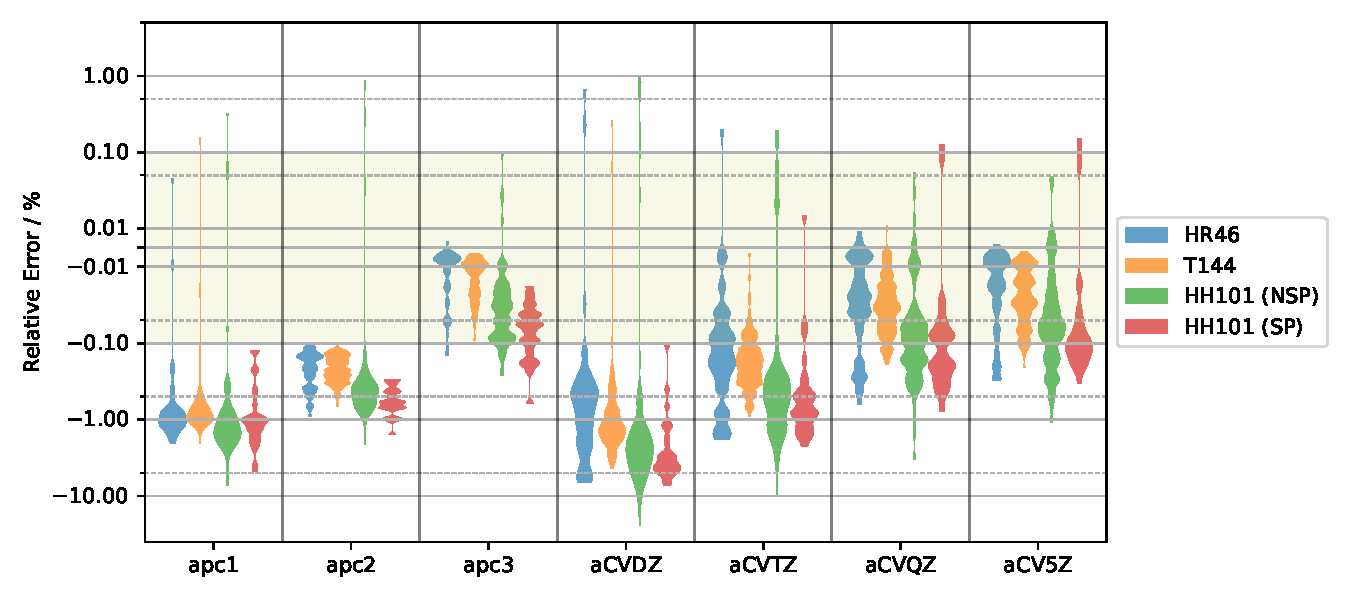
\includegraphics[width=0.9\textwidth]{assets/converg-b2p-scf-apc4.pdf}
    \caption[B2PLYP $\alpha_\textsf{SCF}$ 不同基组相对于 apc4 的相对误差]{B2PLYP 同性极化率的自洽场贡献部分 $\alpha_\textsf{SCF}$ 不同基组相对于 apc4 的相对误差。}
    \label{fig.6.converg-b2p-scf-apc4}
\end{figure}

\subsubsection{B2PLYP 同性极化率二阶微扰部分 $\symup{\Delta} \alpha_\textsf{PT2}$ 的收敛趋势}

图 \ref{fig.6.converg-b2p-pt2-aCV5Z} 与图 \ref{fig.6.converg-b2p-pt2-apc4} 分别展示了以 aCV[Q5]Z 与 apc[34] 作为参考值下 $\symup{\Delta} \alpha_\textsf{PT2}$ 的相对误差收敛趋势。首先,从收敛趋势上,除了 aCVDZ 基组或 HH101 的自旋极化分子集,其余情形绝大多数分子的误差是正误差、且误差确实随基组基数的增大而逐步地逼近零。这表明以 aCV[Q5]Z 与 apc[34] 这两种 CBS 外推模型作为参考值,都有较好的基组收敛性趋势。

\begin{figure}[!t]
    \centering
    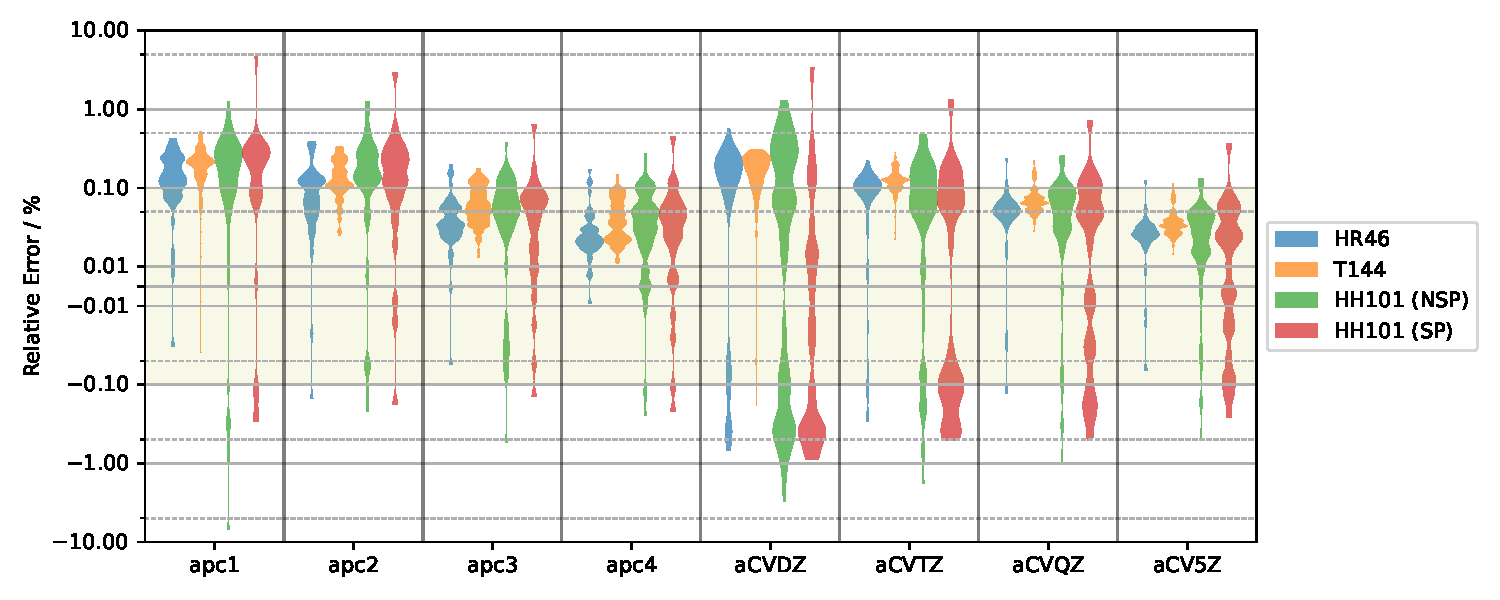
\includegraphics[width=0.9\textwidth]{assets/converg-b2p-pt2-aCV5Z.pdf}
    \caption[B2PLYP $\symup{\Delta} \alpha_\textsf{PT2}$ 不同基组相对于 aCV\text{[Q5]}Z 的相对误差]{B2PLYP 同性极化率的自洽场贡献部分 $\symup{\Delta} \alpha_\textsf{PT2}$ 不同基组相对于 aCV[Q5]Z 的相对误差。}
    \label{fig.6.converg-b2p-pt2-aCV5Z}
\end{figure}

\begin{figure}[!t]
    \centering
    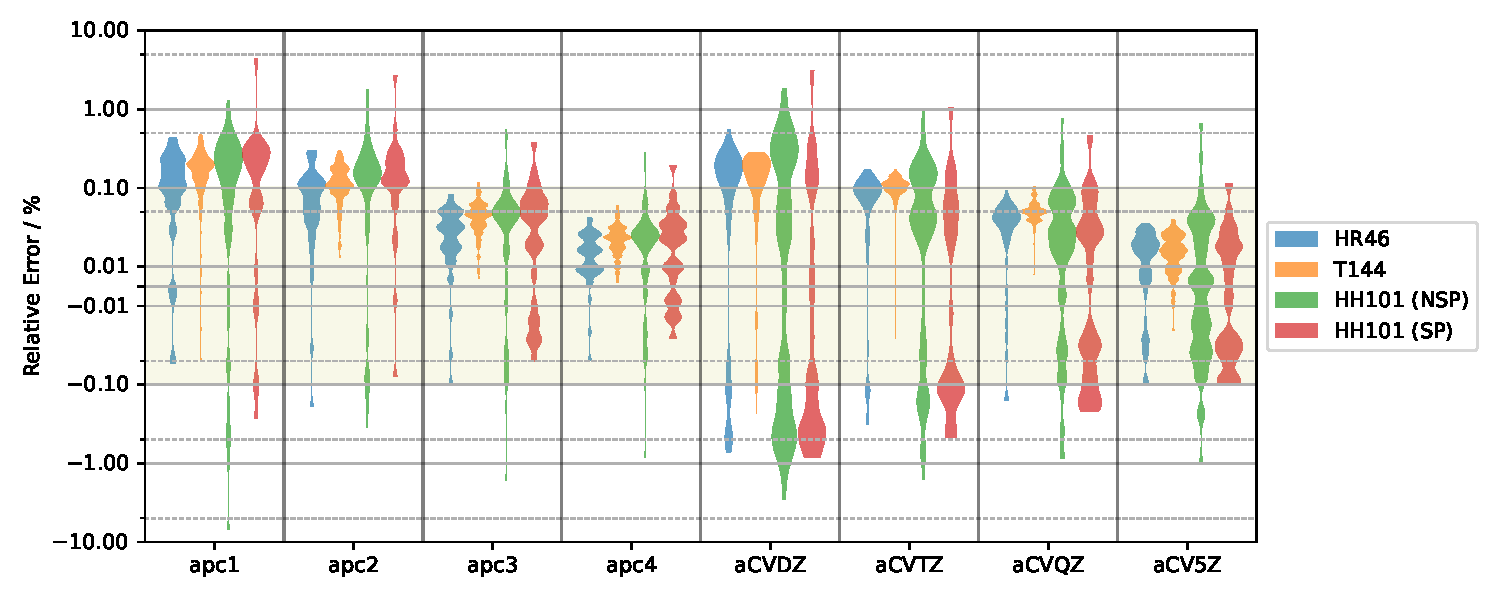
\includegraphics[width=0.9\textwidth]{assets/converg-b2p-pt2-apc4.pdf}
    \caption[B2PLYP $\symup{\Delta} \alpha_\textsf{PT2}$ 不同基组相对于 apc\text{[34]} 的相对误差]{B2PLYP 同性极化率的自洽场贡献部分 $\symup{\Delta} \alpha_\textsf{PT2}$ 不同基组相对于 apc[34] 的相对误差。}
    \label{fig.6.converg-b2p-pt2-apc4}
\end{figure}

但相比于 PBE 泛函可以通过极高精度的 MW7 基组实现 $\alpha_\textsf{SCF}$ 的计算,目前更高基组精度的 $\symup{\Delta} \alpha_\textsf{PT2}$ 计算较为困难;也鲜有在 $\symup{\Delta} \alpha_\textsf{PT2}$ 计算问题上广受验证与测试的高精度 CBS 外推模型\footnote{CBS 外推方法最初是针对相关能而设计的计算方法\cite{Nyden-Petersson.JCP.1981};尽管 CBS 外推方法有长足的发展\cite{Peterson-Dunning.JCP.1994, Nyden-Petersson.JCP.1981, Petersson-Mantzaris.JCP.1988, Jensen-Jensen.TCA.2005, Karton-Martin.TCA.2006, Klopper-Kutzelnigg.JMST.1986, Kutzelnigg-Morgan.JCP.1992, Martin-Martin.CPL.1996, Helgaker-Noga.JCP.1997, Halkier-Wilson.CPL.1998, Halkier-Olsen.CPL.1999},但这些发展通常仍然是提升能量的描述精度。而对于性质的计算,则通常使用与能量计算相同的 CBS 外推模型\cite{Monten-Deleuze.MP.2011, Huzak-Deleuze.JCP.2013, Hait-Head-Gordon.JCTC.2018, Hait-Head-Gordon.PCCP.2018},而鲜有专门针对性质本身设计的 CBS 外推模型。}。同时与 $\alpha_\textsf{SCF}$ 的分析不同,即当使用 apc4 作为 $\alpha_\textsf{SCF}$ 参考值时,基组随基数增大而收敛的趋势比使用 aCV5Z 作为参考值的情形要更加明朗清晰;对于 $\symup{\Delta} \alpha_\textsf{PT2}$,不论使用 aCV[Q5]Z 或 apc[34] 基组的收敛趋势都较为正常。因此,依现有的数据,我们无法判断何种 CBS 外推模型更接近基组极限。

\subsubsection{BSIE 误差的推测}

在正文的工作中,我们主要使用 apc3 基组进行测评计算。在没有基组极限结果的情况下,对于同性极化率 $\alpha_\textsf{DH} = \alpha_\textsf{SCF} + \symup{\Delta} \alpha_\textsf{PT2}$ 的计算,其 BSIE 误差的来源在于
\begin{itemize}[nosep]
    \item 分析基组收敛性时,作为参考值的基组 (5-$\zeta$ 的基组或 CBS 外推模型) 本身的误差;
    \item apc3 与参考值之间的误差。
\end{itemize}

\begin{table}[!t]
\centering
\caption[B2PLYP 泛函 apc\text{[34]} 与 aCV\text{[Q5]}Z 同性极化率的基组 RelRMSD]{B2PLYP 泛函 apc[34] 与 aCV[Q5]Z 外推模型间同性极化率 $\alpha$ 的基组相对方均根误差 (RelRMSD / \%)。}
\label{tab.6.b2p-conv-5zeta}
\widetabular{
    \begin{tabular}{ld{2.4}d{2.4}d{2.4}}
    \toprule
    dataset                & \multicolumn{1}{c}{$\tilde \alpha_\textsf{SCF}$\tnote{b}} & \multicolumn{1}{c}{$\symup{\Delta} \tilde \alpha_\textsf{PT2}$\tnote{c}} & \multicolumn{1}{c}{$\tilde \alpha_\textsf{DH}$\tnote{d}} \\ \midrule
    HR46                   & 0.099 & 0.034 & 0.127 \\
    T144                   & 0.050 & 0.032 & 0.080 \\
    HH101 (NSP)\tnote{a} & 0.214 & 0.154 & 0.282 \\
    HH101 (SP)             & 0.135 & 0.094 & 0.177 \\ \bottomrule
    \end{tabular}
}{
    \item[a] 该误差数据未将氢原子体系纳入统计,即总共分析了 74 个 HH101 数据集的自旋非极化分子体系。
    \item[b] $\text{RelRMSD} (\tilde \alpha_{\textsf{SCF}/\text{apc4}}, \tilde \alpha_{\textsf{SCF}/\text{aCV5Z}}, \tilde \alpha_{\textsf{DH}/\text{aCV[Q5]Z}})$。
    \item[c] $\text{RelRMSD} (\symup{\Delta} \tilde \alpha_{\textsf{PT2}/\text{apc[34]}}, \symup{\Delta} \tilde \alpha_{\textsf{PT2}/\text{aCV[Q5]Z}}, \tilde \alpha_{\textsf{DH}/\text{aCV[Q5]Z}})$。
    \item[d] $\text{RelRMSD} (\tilde \alpha_{\textsf{DH}/\text{apc[34]}}, \tilde \alpha_{\textsf{DH}/\text{aCV[Q5]Z}})$。
}
\end{table}

表 \ref{tab.6.b2p-conv-5zeta} 的数据总结了两种 5-$\zeta$ 级别 CBS 外推模型 apc[34] 与 aCV[Q5]Z 之间的相对误差。首先,对于 $\alpha_\textsf{SCF}$ 的误差,可以看到 HH101 数据集的误差显著地大于 HR46 与 T144 数据集。而 Brakestad 等人工作\cite{Brakestad-Frediani.JCTC.2020}中对 PBE 泛函的误差分析表明,除去两个奇异分子 \ce{^2HO2} 与 \ce{^2Na},其所测评的 HH132 数据集中的 122 个体系 apc4 基组相对于非常接近基组极限的 MW7 基组的相对方均根误差是 0.061\%;远小于我们工作中 B2PLYP 自洽场部分 apc4 与 aCV5Z 之间的 0.214\% (自旋非极化体系) 或 0.135\% (自旋极化体系) 的误差。在假定 B2PLYP 的自洽场部分基组收敛性与 PBE 较为接近的前提下,我们倾向于认为作为 HH132 数据集的子集,HH101 数据集 $\alpha_\textsf{SCF}$ 在 apc4 基组下的相对 BSIE 在 0.06\% 左右;而对于 HR46 与 T144 数据集,apc4 的相对 BSIE 可能更低。对于 $\symup{\Delta} \alpha_\textsf{PT2}$,在没有更精确的基组作为参考值的情况下,我们通过 apc[34] 与 aCV[Q5]Z 之间的相对误差来估计相对 BSIE 大小。对于 HH101 数据集的非自旋极化体系,该相对误差是 0.154\%;其他数据集的相对误差更小。综上,在所测评的数据集、以及 apc[34] 外推模型下,我们预估 B2PLYP 同性极化率 $\tilde \alpha_\textsf{DH}$ 相对 BSIE 将不大于 0.2\%。

\begin{table}[!t]
\centering
\caption[B2PLYP 泛函 apc3 与 aCV\text{[34]}Z 同性极化率的基组 RelRMSD]{B2PLYP apc3 与 apc[34] 间极化率的基组相对方均根误差 (RelRMSD / \%)。}
\label{tab.6.b2p-conv-apc3}
\widetabular{
    \begin{tabular}{lld{2.4}d{2.4}d{2.4}}
    \toprule
    性质 & 数据集 & \multicolumn{1}{c}{SCF} & \multicolumn{1}{c}{PT2} & \multicolumn{1}{c}{DH} \\ \midrule
    同性极化率\tnote{a}     & HR46                   & 0.041 & 0.039            & 0.035 \\
    & T144                   & 0.024 & 0.050            &0.032 \\
    & HH101 (NSP)\tnote{d} & 0.074 & 0.218\tnote{e} & 0.222 \\
    & HH101 (SP)             & 0.159\tnote{f} & 0.095 & 0.145 \\ \midrule
    异性极化率\tnote{b}   & HR46                   & 0.046 & 0.152\tnote{g} & 0.167 \\
    & T144                   & 0.018 & 0.061            & 0.070 \\ \midrule
    极化率分量\tnote{c}    & HH101 (NSP)\tnote{d} & 0.081 & 0.353\tnote{h} & 0.355 \\
    & HH101 (SP)             & 0.165\tnote{i} & 0.101 & 0.153 \\ \bottomrule
    \end{tabular}
}{
    \item[a] 这部分测评的是同性极化率 $\tilde \alpha_\textsf{SCF}, \symup{\Delta} \tilde \alpha_\textsf{PT2}, \tilde \alpha_\textsf{DH}$ 的误差;RelRMSD 误差的具体定义参考表 \ref{tab.6.b2p-conv-hr46-t144-iso} 表头的注释,作为参考值的基组为 apc[34]。
    \item[b] 这部分测评的是异性极化率 $\tilde \gamma_\textsf{SCF}, \symup{\Delta} \tilde \gamma_\textsf{PT2}, \tilde \gamma_\textsf{DH}$ 的误差;RelRMSD 误差的具体定义参考表 \ref{tab.6.b2p-conv-hr46-t144-aniso} 表头的注释,作为参考值的基组为 apc[34]。
    \item[c] 这部分测评的是极化率分量 $\alpha_{xx}, \alpha_{yy}, \alpha_{zz}$ 在自洽场部分、二阶微扰部分、与总和的误差;RelRMSD 误差的具体定义参考表 \ref{tab.6.b2p-conv-hh101-rmsre} 表头的注释,作为参考值的基组为 apc[34]。
    \item[d] 该误差数据未将氢原子体系纳入统计,即总共分析了 74 个 HH101 数据集的自旋非极化分子体系。
    \item[e] \ce{NaCl} 误差为 $-1.660\%$;去除该体系,误差将是 0.102\%。
    \item[f] \ce{^4P} 误差为 $-0.615\%$;去除该体系,误差将是 0.105\%。
    \item[g] \ce{N(CH3)3} 误差为 $-0.622\%$;去除该体系,误差将是 0.117\%。
    \item[h] 去除 \ce{NaCl},误差将是 0.110\%。
    \item[i] 去除 \ce{^4P},误差将是 0.103\%。
}
\end{table}

表 \ref{tab.6.b2p-conv-apc3} 的数据表明,除了一些特例分子 (包括 \ce{NaCl}, \ce{N(CH3)3}, \ce{^4P}),其余情形下 apc3 基组相对于 apc[34],自洽场与二阶微扰两个贡献量的相对误差均不大于 0.1\%;因此,总极化率作为自洽场与二阶微扰贡献量之和,误差不超过 0.2\%。结合上一段的分析,我们认为对于绝大多数分子,apc3 的 BSIE 误差应不大于 0.4\%,处在实验误差 0.5\% 范围以内。

作为这一小节的总结,我们首先注意到了正文的基组收敛性分析中,以 aCV[Q5]Z 为参考值时,以表 \ref{tab.6.b2p-conv-hr46-t144-iso} 为代表的一些测评基准下,存在 apc4 相较于 apc3 误差更大的情形;同时注意到 Brakestad 等人工作\cite{Brakestad-Frediani.JCTC.2020}表明 apc4 的 BSIE 误差相当小,因而引起了我们对 aCV[Q5]Z 作为参考值准确性的疑问、并且希望对 5-$\zeta$ 级别基组或 CBS 外推方法 BSIE 误差作分析。我们从基组的原始 GTO 基函数指数大小、同性极化率误差分布的基组收敛性、以及对比 Brakestad 等人工作\cite{Brakestad-Frediani.JCTC.2020}的结果入手,推断 apc4 相较于 aCV5Z 在 $\alpha_\textsf{SCF}$ 的计算问题上可能具有更低的 BSIE。对于 B2PLYP 泛函,以 apc[34] 作为参考值、并且引入 apc[34] 外推模型的 BSIE 预估值,我们认为绝大多数分子的 apc3 的 BSIE 误差不超过 0.4\%。这与正文中以 aCV[Q5]Z 作为参考值、且未引入 aCV[Q5]Z 的 BSIE 预估值的误差分析结论相仿;因此,使用 apc3 作为双杂化泛函静态极化率的测评基组是合理的。

\subsection{其他补充数据}

\begin{itemize}[nosep]
    \item 表 \ref{tab.6.full-benchmark} 展示了所有经测评密度泛函近似的极化率误差表现。
\end{itemize}

\newpage

\begingroup
\setlength{\LTleft}{-20cm plus -1fill}
\setlength{\LTright}{\LTleft}

\begin{landscape}
\begin{longtable}[c]{lcccccrrrrrrrrc}
\caption[诸密度泛函近似极化率测评表现]{诸密度泛函近似在数据集 HR46、T144 与 HH101 上的极化率测评表现。除 WTRE 为无量纲量外,其余误差以 RelRMSD (\%) 计算${}^a$。}
\label{tab.6.full-benchmark}
\\ \toprule
& & & \multicolumn{3}{c}{杂化类型} & \multicolumn{4}{c}{同性极化率} & \multicolumn{2}{c}{异性极化率} & \multicolumn{2}{c}{极化率分量} & \\
\cmidrule(lr){4-6} \cmidrule(lr){7-10} \cmidrule(lr){11-12} \cmidrule(lr){13-14}
计算方法 & 年代 & 组成 & 交换\tabnote{b} & 相关\tabnote{c} & xDH & \multicolumn{1}{c}{HR46} & \multicolumn{1}{c}{T144} & \multicolumn{2}{c}{HH101} & \multicolumn{1}{c}{HR46} & \multicolumn{1}{c}{T144} & \multicolumn{2}{c}{HH101} & \multicolumn{1}{c}{WTRE} \\
\cmidrule(lr){9-10} \cmidrule(lr){13-14}
& & & & & & & & \multicolumn{1}{c}{NSP} & \multicolumn{1}{c}{SP} & & & \multicolumn{1}{c}{NSP} & \multicolumn{1}{c}{SP} & \\ \midrule
\endfirsthead
\caption[]{(续表)}
\\ \toprule
& & & \multicolumn{3}{c}{杂化类型} & \multicolumn{4}{c}{同性极化率} & \multicolumn{2}{c}{异性极化率} & \multicolumn{2}{c}{极化率分量} & \\
\cmidrule(lr){4-6} \cmidrule(lr){7-10} \cmidrule(lr){11-12} \cmidrule(lr){13-14}
计算方法 & 年代 & 组成 & 交换\tabnote{b} & 相关\tabnote{c} & xDH & \multicolumn{1}{c}{HR46} & \multicolumn{1}{c}{T144} & \multicolumn{2}{c}{HH101} & \multicolumn{1}{c}{HR46} & \multicolumn{1}{c}{T144} & \multicolumn{2}{c}{HH101} & \multicolumn{1}{c}{WTRE} \\
\cmidrule(lr){9-10} \cmidrule(lr){13-14}
& & & & & & & & \multicolumn{1}{c}{NSP} & \multicolumn{1}{c}{SP} & & & \multicolumn{1}{c}{NSP} & \multicolumn{1}{c}{SP} & \\ \midrule
\endhead
\bottomrule
\endfoot
%
XYGJ-OS          & 2011 & GGA  & hyb & hyb & xDH & 0.911 & 0.813 & 1.235  & 1.592  & 2.756  & 1.845  & 1.381  & 1.762  & 0.418 \\
XYG6             & 2021 & GGA  & hyb & hyb & xDH & 1.040 & 1.050 & 1.285  & 1.905  & 2.841  & 2.112  & 1.429  & 2.101  & 0.472 \\
CCSD             &      & WFT  &     &     &     & 1.294 & 1.567 & 1.507  & 1.141  & 2.372  & 2.313  & 1.556  & 1.283  & 0.473 \\
DSD-PBEPBE-D3BJ  & 2013 & GGA  & hyb & hyb &     & 1.146 & 1.274 & 1.615  & 1.412  & 2.234  & 2.446  & 1.651  & 1.578  & 0.473 \\
xDH-PBE0         & 2012 & GGA  & hyb & hyb & xDH & 0.685 & 0.561 & 2.014  & 2.216  & 2.554  & 1.648  & 2.049  & 2.439  & 0.476 \\
XYG-OS5          & 2021 & GGA  & hyb & hyb & xDH & 0.817 & 0.625 & 1.477  & 2.200  & 3.678  & 2.096  & 1.636  & 2.368  & 0.488 \\
ωPBEPP86         & 2021 & GGA  & rsh & hyb &     & 1.093 & 1.069 & 2.068  & 0.949  & 3.252  & 2.542  & 2.090  & 1.074  & 0.490 \\
XYG5             & 2021 & GGA  & hyb & hyb & xDH & 1.095 & 1.138 & 1.330  & 1.981  & 2.739  & 2.235  & 1.479  & 2.197  & 0.490 \\
revXYGJ-OS       & 2021 & GGA  & hyb & hyb & xDH & 0.965 & 0.680 & 1.515  & 2.187  & 3.624  & 2.025  & 1.716  & 2.384  & 0.501 \\
XYG3             & 2009 & GGA  & hyb & hyb & xDH & 1.083 & 1.385 & 1.345  & 2.047  & 2.513  & 3.141  & 1.456  & 2.272  & 0.524 \\
revXYG3          & 2021 & GGA  & hyb & hyb & xDH & 0.971 & 1.062 & 1.739  & 2.410  & 2.493  & 2.671  & 1.858  & 2.645  & 0.540 \\
ωB88PP86         & 2021 & GGA  & rsh & hyb &     & 1.434 & 1.490 & 2.225  & 1.130  & 2.978  & 2.817  & 2.270  & 1.273  & 0.559 \\
ωB2GP-PLYP       & 2019 & GGA  & rsh & hyb &     & 1.062 & 1.140 & 2.374  & 1.829  & 3.005  & 2.824  & 2.403  & 1.875  & 0.569 \\
DSD-PBEP86-D3BJ  & 2013 & GGA  & hyb & hyb &     & 1.720 & 1.826 & 1.974  & 1.317  & 2.563  & 2.714  & 2.032  & 1.420  & 0.574 \\
PBE-QIDH         & 2014 & GGA  & hyb & hyb &     & 1.026 & 1.160 & 2.252  & 1.775  & 3.478  & 3.275  & 2.268  & 1.983  & 0.582 \\
DSD-BLYP-D3BJ    & 2013 & GGA  & hyb & hyb &     & 1.552 & 1.709 & 1.865  & 1.776  & 3.022  & 2.977  & 1.919  & 1.907  & 0.596 \\
SOS0-PBE-QIDH    & 2016 & GGA  & hyb & hyb &     & 1.147 & 1.209 & 2.216  & 2.188  & 3.243  & 2.665  & 2.241  & 2.489  & 0.598 \\
XYG7             & 2021 & GGA  & hyb & hyb & xDH & 2.003 & 1.947 & 2.029  & 1.575  & 2.767  & 2.111  & 2.097  & 1.758  & 0.611 \\
PBE0-2           & 2012 & GGA  & hyb & hyb &     & 1.040 & 0.850 & 2.189  & 3.393  & 3.306  & 2.334  & 2.193  & 3.695  & 0.637 \\
lrc-XYG3         & 2013 & GGA  & hyb & rsh & xDH & 1.294 & 1.733 & 2.405  & 2.020  & 2.799  & 3.565  & 2.479  & 2.260  & 0.651 \\
ωB2PLYP          & 2019 & GGA  & rsh & hyb &     & 1.217 & 1.314 & 2.691  & 2.362  & 3.170  & 3.122  & 2.729  & 2.392  & 0.656 \\
PBE-CIDH         & 2015 & GGA  & hyb & hyb &     & 1.101 & 1.564 & 2.182  & 2.100  & 4.310  & 4.500  & 2.214  & 2.216  & 0.673 \\
RS-B88-LYP       & 2021 & GGA  & rsh & rsh &     & 1.149 & 0.860 & 2.603  & 3.622  & 2.894  & 2.010  & 2.616  & 4.145  & 0.679 \\
LS1DH-PBE        & 2011 & GGA  & hyb & hyb &     & 1.012 & 0.989 & 2.229  & 3.833  & 3.250  & 2.752  & 2.238  & 4.224  & 0.686 \\
B2GP-PLYP        & 2008 & GGA  & hyb & hyb &     & 1.680 & 1.987 & 2.004  & 2.254  & 3.254  & 3.747  & 2.071  & 2.396  & 0.686 \\
SOS0-PBE0-DH     & 2016 & GGA  & hyb & hyb &     & 1.111 & 1.587 & 2.146  & 2.320  & 4.332  & 4.470  & 2.188  & 2.442  & 0.686 \\
TPSS-QIDH        & 2014 & mGGA & hyb & hyb &     & 1.210 & 1.223 & 2.782  & 2.462  & 3.715  & 3.304  & 2.803  & 2.718  & 0.688 \\
RS-PBE-PBE       & 2021 & GGA  & rsh & rsh &     & 1.161 & 0.822 & 2.857  & 3.445  & 3.058  & 1.988  & 2.869  & 4.048  & 0.691 \\
RS-PBE-P86       & 2021 & GGA  & rsh & rsh &     & 1.160 & 0.819 & 2.906  & 3.491  & 3.100  & 2.002  & 2.918  & 4.073  & 0.698 \\
ωB97X-2-TQZ      & 2009 & GGA  & rsh & hyb &     & 1.732 & 1.769 & 2.785  & 2.196  & 2.943  & 2.394  & 2.836  & 2.641  & 0.699 \\
RS-PW91-PW91     & 2021 & GGA  & rsh & rsh &     & 1.223 & 0.853 & 2.937  & 3.474  & 3.094  & 1.986  & 2.950  & 4.080  & 0.706 \\
PBE0-DH          & 2011 & GGA  & hyb & hyb &     & 1.173 & 1.730 & 2.213  & 2.286  & 4.607  & 4.925  & 2.251  & 2.375  & 0.718 \\
PTPSS-D3Zero     & 2011 & mGGA & hyb & hyb &     & 1.823 & 2.138 & 2.385  & 2.477  & 3.131  & 4.104  & 2.450  & 2.530  & 0.749 \\
RSX-QIDH         & 2018 & GGA  & rsh & hyb &     & 1.530 & 1.584 & 3.278  & 2.226  & 4.044  & 3.122  & 3.308  & 2.879  & 0.766 \\
revPBE0-DH       & 2013 & GGA  & hyb & hyb &     & 1.165 & 1.759 & 2.322  & 2.936  & 4.701  & 4.978  & 2.363  & 3.070  & 0.773 \\
TPSS-CIDH        & 2015 & mGGA & hyb & hyb &     & 1.238 & 1.548 & 2.782  & 2.889  & 4.646  & 4.503  & 2.849  & 3.125  & 0.789 \\
TPSS0-DH         & 2013 & mGGA & hyb & hyb &     & 1.241 & 1.662 & 2.760  & 3.028  & 4.953  & 4.910  & 2.805  & 3.252  & 0.819 \\
SOS-RSX-PBE-QIDH & 2021 & GGA  & rsh & hyb &     & 1.821 & 1.933 & 3.331  & 2.662  & 4.408  & 3.197  & 3.370  & 3.398  & 0.848 \\
MPW1K            & 2000 & GGA  & hyb &     &     & 1.654 & 2.024 & 2.899  & 2.426  & 5.929  & 5.502  & 2.971  & 2.663  & 0.877 \\
mPW2PLYP         & 2006 & GGA  & hyb & hyb &     & 2.255 & 2.678 & 2.647  & 3.273  & 3.948  & 4.853  & 2.762  & 3.431  & 0.918 \\
SCAN0            & 2016 & mGGA & hyb &     &     & 1.718 & 2.551 & 2.504  & 2.668  & 6.328  & 7.160  & 2.608  & 2.857  & 0.946 \\
RSX-0DH          & 2019 & GGA  & rsh & hyb &     & 2.047 & 2.251 & 3.968  & 2.683  & 5.429  & 4.062  & 4.017  & 3.531  & 0.979 \\
PBE50            & 2012 & GGA  & hyb &     &     & 2.108 & 2.226 & 3.398  & 2.839  & 6.371  & 5.224  & 3.475  & 3.114  & 0.985 \\
MP2              &      & WFT  &     &     &     & 2.609 & 0.813 & 2.146  & 4.752  & 10.532 & 1.625  & 2.188  & 5.693  & 0.994 \\
B2PLYP           & 2006 & GGA  & hyb & hyb &     & 2.552 & 2.987 & 2.908  & 3.468  & 4.256  & 5.194  & 2.998  & 3.656  & 1.002 \\
SOS-RSX-PBE0-DH  & 2021 & GGA  & rsh & hyb &     & 2.188 & 2.401 & 4.005  & 2.850  & 5.618  & 4.096  & 4.058  & 3.737  & 1.016 \\
M11              & 2011 & mGGA & rsh &     &     & 1.490 & 1.859 & 4.525  & 4.341  & 5.459  & 5.046  & 4.682  & 5.799  & 1.117 \\
MVS              & 2015 & mGGA &     &     &     & 1.658 & 2.550 & 3.460  & 2.823  & 7.291  & 9.230  & 3.659  & 3.694  & 1.124 \\
CAM-B3LYP        & 2004 & GGA  & rsh &     &     & 2.315 & 2.612 & 4.080  & 4.621  & 4.286  & 5.258  & 4.184  & 4.733  & 1.127 \\
PBE0             & 1999 & GGA  & hyb &     &     & 2.478 & 3.247 & 3.874  & 4.148  & 6.272  & 7.493  & 3.979  & 4.243  & 1.232 \\
M06-2X           & 2006 & mGGA & hyb &     &     & 1.548 & 1.930 & 3.310  & 8.244  & 5.741  & 4.998  & 3.394  & 8.438  & 1.242 \\
MN15             & 2016 & mGGA & hyb &     &     & 2.613 & 2.892 & 3.366  & 7.328  & 4.785  & 6.037  & 3.500  & 7.908  & 1.324 \\
mBEEF            & 2014 & mGGA &     &     &     & 2.501 & 3.714 & 3.588  & 4.523  & 8.951  & 10.585 & 3.771  & 4.662  & 1.408 \\
M06              & 2006 & mGGA & hyb &     &     & 2.488 & 3.282 & 4.622  & 7.004  & 7.030  & 8.107  & 4.756  & 7.175  & 1.507 \\
ωB97M-V          & 2016 & mGGA & hyb &     &     & 3.188 & 3.207 & 5.395  & 8.415  & 4.615  & 4.898  & 5.555  & 8.627  & 1.555 \\
SCAN             & 2015 & mGGA &     &     &     & 3.410 & 4.485 & 4.688  & 4.841  & 8.410  & 10.529 & 4.792  & 5.153  & 1.597 \\
M06-L            & 2006 & mGGA &     &     &     & 1.847 & 3.131 & 3.835  & 9.348  & 7.531  & 9.761  & 4.118  & 9.793  & 1.614 \\
TPSSh            & 2003 & mGGA & hyb &     &     & 3.362 & 4.396 & 4.966  & 5.497  & 7.975  & 9.892  & 5.070  & 5.628  & 1.619 \\
B3LYP            & 1993 & GGA  & hyb &     &     & 3.790 & 4.524 & 5.195  & 6.111  & 6.646  & 8.458  & 5.381  & 6.369  & 1.647 \\
HF               &      & WFT  &     &     &     & 4.727 & 4.126 & 6.592  & 5.948  & 13.901 & 8.483  & 6.868  & 7.069  & 1.986 \\
TPSS             & 2003 & mGGA &     &     &     & 4.875 & 5.916 & 6.843  & 7.721  & 10.162 & 12.239 & 6.998  & 8.071  & 2.198 \\
N12              & 2012 & GGA  &     &     &     & 4.666 & 5.446 & 7.607  & 11.687 & 11.588 & 13.180 & 8.072  & 12.043 & 2.535 \\
MPW91            & 1998 & GGA  &     &     &     & 6.042 & 6.860 & 8.515  & 10.081 & 11.414 & 13.041 & 8.712  & 11.005 & 2.665 \\
PBE              & 1997 & GGA  &     &     &     & 6.690 & 7.369 & 9.403  & 11.117 & 12.088 & 13.202 & 9.652  & 12.131 & 2.890 \\
BLYP             & 1988 & GGA  &     &     &     & 7.446 & 8.153 & 10.425 & 12.666 & 12.103 & 13.292 & 10.752 & 13.838 & 3.164
\end{longtable}
\vspace{-1em}
\footnotesize
\par\noindent\emph{a} 该表格以 WTRE 数值排序。作为参考值的方法是 CCSD(T);如前文所述,HH101 参考值由 Hait 与 Head-Gordon 在 aCV[TQ]Z 或 aCV[Q5]Z 级别下给出\cite{Hait-Head-Gordon.PCCP.2018};HR46 与 T144 参考值由本论文第 \alertref{sec.5.title} 章给出,为 FPA-aV[DT]Z、FPA-aV[TQ]Z 或 FPA-aV[Q5]Z 级别下给出。
\par\noindent\emph{b} “hyb”指交换能中掺杂部分非局域的严格交换能;“exact”指交换能全部为严格交换能;“rsh”指交换能包含长短程分离的非局域交换能,不论其是否包含非局域短程交换。该项若非空缺,则视为杂化泛函。
\par\noindent\emph{c} “hyb”指相关能中掺杂 MP2 型非局域相关能;“rsh”指相关能中掺杂长短程分离的 MP2 型非局域相关能。该项若非空缺,则视为双杂化泛函。
\end{landscape}

\endgroup
